\chapter{The State of the Art}

In the following chapter we will briefly go through the knowledge we acquired while exploring already existing materials in the same context of our problem.

\section{Sentiment Analysis} 
Sentiment Analysis (SA) is the computational study of people's opinions, attitudes and emotions toward an entity, the entity being an individual, event or topic.\cite{survey} \par

Sentiment Analysis can be considered a classification task as illustrated in Fig \ref{fig:sa_process}.\\

\begin{figure}[H]
\centering
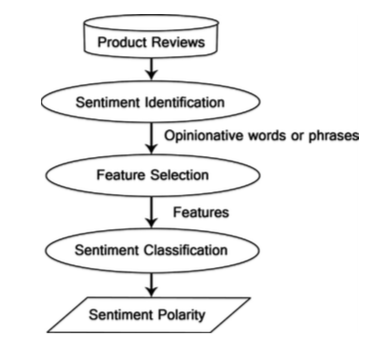
\includegraphics[width=0.4\textwidth]{./chapters/chapter1/images/sa_process}
\caption{Sentiment analysis process on product reviews\cite{survey}}
\label{fig:sa_process}
\end{figure}

There are three main classification levels in SA: 
\begin{itemize}
\item Document-level
\item Sentence-level
\item Aspect-level
\end{itemize}
Their difference is the granularity at which they operate. Indeed, while document-level SA aims to classify a document as expressing a positive or negative opinion or sentiment by considering the whole document as the basic information unit, sentence-level SA aims at classifying the sentiments/opinions expressed in each sentence.
In both cases the first step is to identify whether the sentence/document is subjective or objective and if it is subjective determine whether the sentence expresses positive or negative opinions. \par

In certain applications, classifying text at the document level or at the sentence level may not provide the necessary details needed for detecting opinions on all aspects of the entity. Aspect-level SA, instead, aims at classifying the sentiment with respect to the specific aspects of entities. The first step is to identify the entities and their aspects. Then, all the different opinions on the same entity must be considered. Indeed, the opinion holders may also give different opinions for different aspects of the same entity, e.g. ``This chair is ugly but it is comfortable''.

Sentiment Analysis task is considered as a sentiment classification (SC) problem. The first step in the SC problem is to extract and select text features. Some of the most commonly used features are:
\begin{itemize}
\item \textbf{Terms presence and frequency}: These features are individual words or word n-grams and their frequency counts;
\item \textbf{Parts of speech (POS)}: finding adjectives, pronouns, etc. as they are important indicators of opinions;
\item \textbf{Opinion words and phrases}: these are words commonly used to express opinions including \textit{good or bad, like or hate}. On the other hand, some phrases express opinions without using opinion words, e.g. \textit{cost me and arm and a leg};
\item \textbf{Negations}: the appearance of negative words may change the opinion orientation like \textit{not good} is equivalent to \textit{bad}. 
\end{itemize}

Sentiment Classification techniques can be roughly divided into machine learning approach, lexicon based approach and hybrid approach\cite{survey}. \par

The \textit{Machine Learning Approach (ML)} applies the famous ML algorithms and uses linguistic features. 

The \textit{Lexicon-based Approach} relies on a sentiment lexicon, a collection of known and precomiled sentiment terms. It is divided into dictionary-based approach and corpus-based approach which use statistical or semantic methods to find sentiment polarity.

The \textit{Hybrid Approach} combines both approaches. 

The various approaches and the most popular algorithms of SC are illustrated in Fig \ref{fig:sentiment_classification}. 

\begin{figure}[H]
\centering
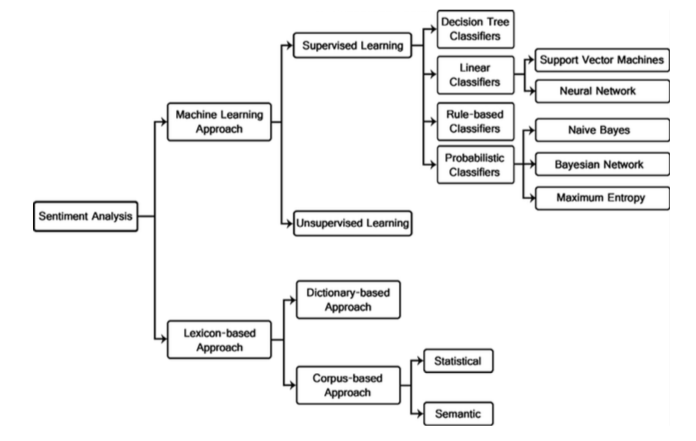
\includegraphics[width=0.8\textwidth]{./chapters/chapter1/images/sentiment_classification}
\caption{Sentiment classification techniques\cite{survey}}
\label{fig:sentiment_classification}
\end{figure}

The text classification methods using ML approach can be roughly divided into supervised and unsupervised learning methods. The supervised methods make use of a large number of labeled training documents. The unsupervised methods are used when it is difficult to find these labeled training training documents. \par
The lexicon-based approach depends on finding the opinion lexicon which is used to analyze the text. There are two methods in this approach:

\begin{itemize}
\item Dictionary-based
\item Corpus-based
\end{itemize}

In the Dictionary-based approach a small set of opinion words is collected manually with known orientations. Then, this set is grown by searching their synonyms and antonyms. The newly found words are added to the seed list then the next iteration starts. The iterative process stops when no new words are found. The dictionary based approach has a major disadvantage which is the inability to find opinion words with domain and context specific orientation. 

The limitation of the dictionary-based approach is addressed by the corpus-based approach, which depends on syntactic patterns or patterns that occur together along with a seed list of opinion words to find other opinion words in a large corpus. One of these methods is called \textit{sentiment consistency}: it starts with a list of seed opinion adjectives, and used them along with a set of linguistic constraints to identify additional adjective opinion words and their orientations. The constraints being for example \textit{AND, OR, BUT, EITHER-OR,...}; the conjunction \textit{AND} for example says that conjoined adjectives usually have the same orientation. \par

\section{Emotion Detection}

Emotion detection (ED) is the process of identifying human emotions. It is a recent field of research that is closely related to Sentiment Analysis. Indeed, Sentiment Analysis aims to detect positive, neutral or negative feelings from text, whereas Emotion Analysis aims to detect and recognize feelings in natural language texts. Therefore we can look at ED as a finer grained task with respect to SA.\par
Emotion is expressed as joy, sadness, anger, surprise, hate, fear and so on. Since there is not any standard emotion word hierarchy, the focus is on the related research about emotion in cognitive psychology domain. In 2001, W. Gerrod Parrot, wrote a book named ``Emotions In Social Psychology''\cite{Parrott2016}, in which he explained the emotion system and formally classified the human emotions through an emotion hierarchy in six classes at primary level which are \textit{Love, Joy, Anger, Sadness, Fear and Surprise} \cite{edfromtext}.\par

Emotion detection may have useful applications, such as \cite{microsoft}: 
\begin{itemize}
\item Measure citizens happiness;
\item Pervasive computing: this may include suggesting help when anxiety is detected through speech, or to check the tone of an email; 
\item Improving perception of a customer to increase brand reputation and sales. 
\end{itemize}

Some of the biggest challenges in determining emotion are:
\begin{itemize}
\item \textit{Context-dependence of emotions}: people use different regulation strategies in different social contexts. A phrase can have element of \textit{anger} without using the word ``anger'' or any of its synonyms, e.g. \textit{``Shut up!''}
\item \textit{Word-sense disambiguation}: identifying which sense a word (i.e. its meaning) is used in a sentence, when the word has multiple meanings; 
\item \textit{Co-reference resolution}: pronouns and other referring expressions must be connected to the right individuals;
\item Lack of labelled emotion databases. 
\end{itemize}

The main methods used for text based emotion detection are\cite{emodetect-from-text}: 
\begin{itemize}
\item \textit{Keyword Spotting}
\item \textit{Lexical Affinity}
\item \textit{Learning-based}
\item \textit{Hybrid}
\end{itemize}

\paragraph{Keyword Spotting}
The keyword pattern matching problem can be described as the problem of finding occurrences of keywords from a given set as substrings in a given string. These words are classified into categories such as disgusted, sad, happy, angry, fearful, surprised, etc. The process of Keyword spotting method is  shown in Fig \ref{fig:keyword_spotting}. 

\begin{figure}[H]
\centering
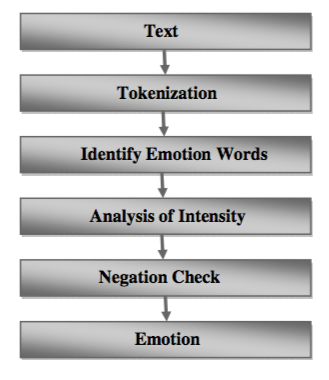
\includegraphics[width=0.4\textwidth]{./chapters/chapter1/images/keyword_spotting}
\caption{Keyword spotting technique}
\label{fig:keyword_spotting}
\end{figure}

The first step is converting data into tokens, i.e. a sentence into words, then from these tokens emotion words are detected. The second step is analyzing the intensity of emotion words. Sentence, then, is checked whether negation is involved in it or not then finally an emotion class will be assigned.

\paragraph{Lexical Affinity method} 
The Lexical Affinity approach is an extension of keyword spotting technique: apart from picking up emotional keywords it assigns \textit{probabilistic affinity} for a particular emotion to arbitrary words. This technique has the main disadvantage of missing out emotion content that resides deeper than the word level.\\
For example the word 'accident', having been assigned a high probability of indicating a negative emotion, would not contribute correctly to the emotional assessment of phrases like \textit{``I avoided an accident''} or \textit{``I met my girlfriend by accident''}. 

\paragraph{Learning-based methods}
Learning-based methods change the focus from ``determining emotions'' to ``classify the input texts into different emotions''. Indeed, learning-based methods try to detect emotions based on a previously trained classifier, which apply various theories of machine learning such as Support Vector Machines (SVMs).

\paragraph{Hybrid Methods}
Since keyword-based methods and na\"{i}ve learning-based methods could not acquire satisfactory results, some systems use hybrid approach by combining both keyword spotting technique and learning based method, which help to improve accuracy. \\
\\

However all these methods have some major limitations:
\begin{itemize}
\item \textit{Ambiguity in Keyword Definitions}: words can have multiple and vague meanings that can change according to different usages and contexts. Moreover emotion labels could have different emotions in some extreme cases such as ironic or cynical sentences; 
\item \textit{Lack of Linguistic Information}: these methods totally ignore syntax structures and semantics that also have influences on expressed emotions. For example the sentences \textit{``He laughed at me''} or \textit{``I laughed at him''} express two totally different meanings;
\item \textit{Incapability of Recognizing Sentences without Keywords}: sentences without any keyword would imply that they do not contain any emotion at all, which is obviously wrong. 
\end{itemize}

Deciding a way to label emotions is another challenging aspect of ED. There are mainly two possible ways to label data \cite{microsoft}:
\begin{enumerate}
\item The label is one between the set of emotions, e.g. \textit{anger, disgust, sad, happy, surpise, fear, neutral};
\item \textit{Slider approach}: the label is composed of percentages for each emotion, as described in Fig \ref{fig:emotion_labeling_sliders}.
\end{enumerate}

\begin{figure}[H]
\centering
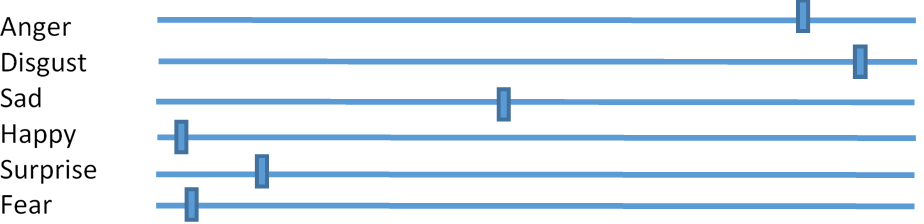
\includegraphics[width=0.8\textwidth]{./chapters/chapter1/images/emotion_labeling_sliders}
\caption{Slider approach\cite{microsoft}}
\label{fig:emotion_labeling_sliders}
\end{figure}

The sliders approach certainly offers more information but it comes with additional computational complications. However, the probabilistic assignment produced in the sliders approach can be turned into distinct labels of single emotions, just like those produced by first labeling approach, but of course, we can not move from the first approach to the second one. 

